\documentclass[UTF8,a4paper,zihao=-4]{ctexart}

\usepackage{amsmath,amssymb}
\usepackage{booktabs}
\usepackage{tabularx}
\usepackage{array}
\usepackage{graphicx}
\usepackage{float}
\usepackage{enumitem}
\usepackage{hyperref}
\usepackage{caption}
\usepackage{geometry}

% CUMCM 2026 default paper typography and spacing.
% Requires XeLaTeX, ctex, geometry, fontspec, and booktabs.
% Recommended class option for the current template profile:
% \documentclass[UTF8,a4paper,zihao=-4]{ctexart}
\geometry{top=2.5cm,bottom=2.5cm,left=2.5cm,right=2.5cm}
% The 2026 format does not require a running header. Keep the required page
% number in the centered footer instead of inheriting ctexart's headings style.
\pagestyle{plain}
\setmainfont{Times New Roman}
\setCJKmainfont[BoldFont=SimHei]{SimSun}
% Keep mathematics in XeLaTeX's single Computer Modern family; do not mix a
% second math-font package into the manuscript unless the entire paper is
% rechecked for consistent glyph metrics.
\AtBeginDocument{\zihao{-4}}
\setlength{\parindent}{2em}
\setlength{\parskip}{0pt}
\ctexset{
  section={name={,、},number=\chinese{section},format=\centering\zihao{3}\bfseries,afterindent=true},
  subsection={format=\zihao{4}\bfseries,afterindent=true},
  subsubsection={format=\zihao{-4}\bfseries,afterindent=true}
}
% Keep a figure-only page aligned to the top instead of vertically centering it.
\makeatletter
\setlength{\@fptop}{0pt}
\makeatother

% Abstract/body emphasis policy: headings and short question leads may be bold;
% ordinary scientific prose, assumptions, derivations, and table discussion
% remain regular weight.  Keep \CUMCMAbstractKey for short, selective anchors
% only; never wrap a full sentence or paragraph in it.
% Abstract-page semantics. These avoid the implicit \small used by many
% standard abstract environments.
\newcommand{\CUMCMTitle}[1]{%
  \begin{center}{\zihao{3}\bfseries #1\par}\end{center}%
}
\newcommand{\CUMCMAbstractHeading}{%
  \begin{center}{\zihao{4}\bfseries 摘\quad 要\par}\end{center}%
}
\newcommand{\CUMCMAbstractParagraph}{\par\indent}
\newcommand{\CUMCMAbstractLead}[1]{\par\indent\textbf{针对问题#1，}}
\newcommand{\CUMCMAbstractKey}[1]{{\bfseries\boldmath #1}}
\newcommand{\CUMCMKeywords}[1]{\par\noindent\textbf{关键词：}#1}
\newcommand{\CUMCMQuestionLead}[1]{\par\indent\textbf{问题#1：}}
\newcommand{\CUMCMAnalysisLead}[1]{\par\indent\textbf{问题#1：}}


\hypersetup{
  hidelinks,
  pdftitle={时频资源离散化与字典序整数优化的装备用频冲突检测与消解}
}

\begin{document}

\CUMCMTitle{时频资源离散化与字典序整数优化的装备用频冲突检测与消解}
\CUMCMAbstractHeading
\begingroup
\zihao{-4}
\CUMCMAbstractParagraph
面向 150 条具有重复占用结构的装备用频计划，需要依次完成冲突检测、冲突消解、固定方案下的新增容量评估，以及允许改变重复间隔后的再优化。统一采用“计划—重复事件—时频资源格”三层表示：先按半开区间展开全部使用事件，再把二维几何相交转化为离散资源互斥。四问由精确检测、条件字典序优化、集合装填和间隔扩展依次衔接，并用独立编码和阈值不可行证据核验关键结论。

\CUMCMAbstractLead{一}建立\CUMCMAbstractKey{半开区间二维相交模型}，采用“频段预筛—完整事件枚举”算法：只有两个计划的频段相交，且至少一对重复事件的时间区间相交时，才记录一条计划层冲突边；另以离散资源格倒排索引独立重建冲突图。150 条计划展开为 1\,300 个事件，枚举 11\,175 个候选计划对，得到 297 对冲突装备和 431 次事件级重叠；其中 B--C 类有 181 对，类别内冲突率为 5.03\%。

\CUMCMAbstractLead{二}把保留、频移、时移和撤销统一为互斥候选动作，建立\CUMCMAbstractKey{候选动作资源格互斥 0--1 模型}；采用 CP-SAT 求解主模型，再用独立 CNF 编码和 CaDiCaL 对“更优一档”进行阈值不可行检验。4\,582 个合法动作由 52\,939 条资源格团约束控制，并按\CUMCMAbstractKey{条件字典序}逐层固定目标，闭合前缀为 \CUMCMAbstractKey{$(R,R_A,R_B,M,M_A,M_B)=(6,0,4,126,16,34)$}，即撤销 6 条、调整 126 条。末级平移量 $S_{10}=775$ 仅是该前缀下的可行上界。

\CUMCMAbstractLead{三}固定问题二验证后的 144 条活动计划，完整枚举 52\,136 个 C 类整数起点，筛得 2\,334 个与既有占用不冲突的候选；随后建立\CUMCMAbstractKey{0--1 集合装填模型}，用 HiGHS 最大化新增数量。资源格装填编码与独立的候选两两冲突编码均得到 \CUMCMAbstractKey{最多新增 141 台}，且加入“至少 142 台”约束后模型不可行。该最大值只适用于当前 Q2 方案、资源域 \([0,643)\times[0,100)\) 和给定 C 类模板。

\CUMCMAbstractLead{四}从原始 150 条计划独立起算，为 C 类加入整数间隔动作，构建\CUMCMAbstractKey{间隔扩展资源格模型}。基准域生成 6\,103 个合法动作，经外部冲突集合支配消元后，对 \(R=2\) 的六种类别分拆分别建立 SAT 判定模型；CP-SAT 给出 3 台撤销可行见证，CaDiCaL 证明六个两撤销分支均不可行，由上下界闭合得到 \CUMCMAbstractKey{最少撤销 3 台}。该结论限于 \(H=643\) 和当前有限整数动作集合；142 个调整及末级变化量 943 仍是条件候选。

连续半开区间检查与离散资源格检查在四问中一致，调整方案均满足零冲突、零越界和资源格单占用；\(H=638,643,648\) 的复核表明 Q2 最小撤销数均为 6，并支持 Q4 三撤销可行上界对边界扰动稳定。上述模型链把重复事件的几何关系转化为可复核的整数约束，同时明确保留 Q2 末级平移量和 Q4 次级目标尚未闭合的证据边界。
\CUMCMKeywords{时频资源；冲突检测；条件字典序；0--1 整数优化；集合装填}
\endgroup
\clearpage

\section{问题重述}
\subsection{问题背景}

题目研究有限时频资源下的装备用频编排。系统提供 100 个离散频段，现有 150 条用频计划分为 A、B、C 三类，优先级依次降低。每条计划由频段区间、首次使用时间区间、间隔时长和使用次数定义，并沿时间轴重复占用同一频段；若两条计划的频段区间相交，且至少有一对重复事件的时间区间也相交，则发生时频冲突。因此，判定冲突不能只比较首次时间区间，而要先还原完整重复事件，再在统一的时间—频率边界内处理计划之间的资源关系。

\subsection{问题提出}

前三问构成一条依赖链：先识别冲突，再按有限调整规则和类别优先级消解冲突，最后固定方案并计算新增 C 类计划。各问的“最多”均限定在题目给定的资源域、动作模板和冻结输入内；第四问允许改变 C 类计划的间隔时长，本阶段暂不运行。

\CUMCMQuestionLead{一}
对原始计划逐条展开其全部重复使用事件，并判定任意两条计划是否存在冲突。冲突采用两个维度同时满足的口径：频段区间有交集，且至少有一对重复事件的时间区间有交集。时间区间使用半开形式，左端点计入、右端点不计入，以避免首尾相接被误判为重叠。该问的直接输出是计划层的冲突装备对清单；事件级重叠次数作为辅助核验量保留。除计划对枚举外，还需要用离散时频资源格重新检查同一结果，从而区分“冲突装备对数”和“发生重叠的事件次数”这两个统计口径。

\CUMCMQuestionLead{二}
在问题一得到的冲突背景下，为每条原计划选择一种动作：保持不变、频率平移、时间平移或撤销。频率平移量和时间平移量分别受到给定范围限制，一条计划不能同时改变两个维度，调整后全部重复事件仍须落在资源域内，并且所有计划之间不得共享同一时频资源格。题面只说明“尽量少撤销、尽量少调整并优先保护高等级装备”，没有给出可直接相加的数值权重，因此需要把这些要求转化为可审计的条件字典序。输出不仅包括一份无冲突动作表，还要给出每一层优先目标的可行解、下界和不可行阈值证据；其中末级平移量若只得到当前可行上界，必须单独标注其证明边界。

\CUMCMQuestionLead{三}
固定问题二通过验证的具体方案，不再重新移动或撤销其中的既有计划。在同一时间—频率资源域内，按照附件给出的 C 类装备共同结构生成所有可能的新增起点，逐个展开其完整重复事件，删除与固定问题二背景发生冲突的候选，再从剩余候选中选出数量最多且彼此不冲突的一组。该问的输出是最大新增数量及相应新增计划表；“最大”仅针对当前冻结的 Q2 方案、当前资源域和 C 类模板成立。为避免结果依赖某一种约束编码，需要用资源格集合装填模型和候选两两冲突模型交叉验证最大值，并单独检查新增计划与原有方案之间的边界和重复占用。

\CUMCMQuestionLead{四}
第四问允许改变 C 类计划的间隔时长，会重新改变事件递推关系；本阶段暂不运行，因此不改写问题一至问题三的输入和结论。

\clearpage

\section{问题分析}
问题分析围绕共同的资源表示展开。原始计划按频段、首次时间、间隔和次数展开为完整重复事件，再映射到时间—频率资源格；计划层识别冲突，事件层记录重叠次数，资源格层写出互斥约束。三层表示相互对应：Q1 的冲突边传给 Q2，Q2 的验证方案成为 Q3 的冻结背景，所有结果回溯同一份预处理结果。

\CUMCMAnalysisLead{一}
关键是把计划记录还原为可比较的事件集合。对第 $i$ 条计划，依据首次使用时刻、单次时长、间隔和次数递推全部事件，统一采用半开时间区间。先用频段区间相交筛选计划对，再检查候选对中是否存在时间相交的重复事件；计划层只保留一条无向冲突边，事件级重叠次数另行保存。随后把事件占用转换为离散资源格，用倒排关系复核冲突清单。150 条计划展开 1\,300 个事件，枚举 11\,175 个候选对，得到 297 对冲突装备和 431 次事件级重叠，其中 B--C 类为 181 对。输出的冲突图同时作为问题一结果和问题二硬约束输入。

\CUMCMAnalysisLead{二}
难点是把“少撤销、保护高等级、少调整”变成可审计的优先级。对每条计划生成保持、频移、时移和撤销候选；候选均重新展开事件并形成资源格集合，越界者先剔除。一条计划只能选一种动作，一个资源格至多由一个候选使用，于是得到 0--1 资源格模型。目标不采用未经授权的加权和，而按 $(R,R_A,R_B,M,M_A,M_B,S_{10})$ 逐层固定；每层记录可行值、下界或阈值不可行证据，只有上下界闭合才写成已证明结论。4\,582 个合法候选动作对应 52\,939 条资源格团约束，前六层闭合为 $(6,0,4,126,16,34)$；$S_{10}=775$ 仍只是该前缀下的可行上界。连续区间与离散资源格回读均零冲突，144 个活动计划及 15\,816 个占用格成为问题三的冻结输入。

\CUMCMAnalysisLead{三}
研究固定问题二方案后的剩余容量，不允许新增计划反向改变 Q2 布局。继承 Q2 的 144 个活动计划及其资源格占用，按 C 类共同结构枚举合法的时间起点和频段起点；每个起点均展开完整事件，并通过资源域和固定背景冲突检查。候选按逐格占用筛选，而不是用剩余面积估计；随后用资源格集合装填和候选两两冲突两种编码交叉求解。52\,136 个完整 C 类起点中有 2\,334 个与冻结背景不冲突，两种模型均得到 141 台新增计划，且“至少 142 台”不可行。因此，141 只是在当前 Q2、资源域和 C 类模板下的最大值。

\CUMCMAnalysisLead{四}
问题四的变化不在于重新定义冲突，而在于放开 C 类计划的重复间隔。间隔一旦改变，第二次及以后的所有事件都会联动移动，因此不能只修补某一个事件，也不能用平均占用量代替完整展开。处理方式是从问题一的 150 条原始计划独立起算，枚举保持、频移、时移、撤销以及 C 类间隔调整动作；对每个动作递推全部事件，先剔除越界候选，再用资源格互斥约束统一判定。这样可把“允许更灵活的周期结构”转化为有限的整数动作集合。基准域共生成 6\,103 个合法候选动作，支配替换后保留 5\,533 个活动候选。3 台撤销的可行见证与 2 台及以下六种类别分支的不可行证据分别形成上下界，闭合当前有限模型下的最小撤销层。需要特别区分的是，$R=3$ 之外的类别撤销、调整数量和末级变化量仍只是当前条件候选，不能因求解器返回可行解就改写为完整字典序最优。

四问接口由预处理和边界验证共同固定：原始字段只在预处理阶段解释一次，重复事件采用同一半开区间，资源格使用同一时间域和频段域。Q2 的 $H=638,643,648$ 检验均给出最小撤销数 6；Q4 在三个边界情景均找到通过验证的三撤销候选。由此，Q1 的冲突事实、Q2 的条件字典序方案、Q3 的固定背景最大值和 Q4 的最小撤销层形成可追踪证据链，各问仍按照各自的输入接口和证明范围报告。


\section{模型假设与符号说明}
\subsection{模型基本假设}
模型假设只保留会改变冲突判定、候选生成或跨问接口的规则，具体如下。

\begin{enumerate}[label=(\arabic*), leftmargin=*, itemsep=0.35em, topsep=0.25em, parsep=0pt]
  \item 区间与离散单位。时间区间和频段区间均采用半开区间，只有内部存在正长度交集才判定为重叠；原始端点及调整量按题面给出的离散单位取整数。该口径使首尾相接的事件不产生虚假冲突，并使连续区间检查能够与资源格复核逐格对应。\label{ass:interval}
  \item 重复事件与动作规则。一份计划的全部重复事件共享频段区间，频移或时移同时作用于该计划的全部事件；问题二中每份计划至多选择保留、频移、时移或撤销中的一种动作，并保持单次时长、间隔时长和使用次数不变。\label{ass:action}
  \item 跨问接口与 Q4 范围。问题二和问题三的基准资源域取 \([0,643)\times[0,100)\)，问题三冻结已经验证的问题二具体方案并采用频段宽 3、单次时长 2、间隔 8、使用 12 次的 C 类模板；问题四从问题一的 150 条原始计划独立起算，只允许 C 类计划取整数间隔 \(g_i'\in\{0,1,\ldots,18\}\)，不叠加频移或时移，也不读取 Q2 撤销和 Q3 新增计划。\label{ass:cross-interface}
\end{enumerate}

资源域、新增模板和问题四的间隔范围是为保证跨问一致性与可验证性而采用的明确建模口径；相关结果均在正文中标注其适用范围。


\clearpage
\subsection{符号说明}
\begin{table}[htbp]
\centering
\small
\renewcommand{\arraystretch}{0.92}
\caption{符号说明}
\label{tab:symbols}
\begin{tabularx}{0.94\textwidth}{>{\centering\arraybackslash}p{0.24\textwidth} X}
\toprule
符号 & 含义 \\
\midrule
\(\mathcal I\) & 原始用频计划集合，包含 150 份计划。\\
\(i,j\) & 用频计划或装备的索引。\\
\(k\) & 同一计划内重复事件的序号。\\
\([f_i^-,f_i^+)\) & 计划 \(i\) 的频段半开区间，端点按离散频率单位记录。\\
\([s_i,e_i)\) & 计划 \(i\) 的首次时间半开区间，端点按离散时间单位记录。\\
\(l_i\) & 计划 \(i\) 的单次使用时长，满足 \(l_i=e_i-s_i\)。\\
\(g_i\) & 计划 \(i\) 的空闲间隔时长。\\
\(n_i\) & 计划 \(i\) 的重复使用次数。\\
\(E_i\) & 计划 \(i\) 展开后的完整重复事件集合。\\
\(C_{ij}\) & 计划 \(i\) 与计划 \(j\) 是否存在时频冲突的指示量。\\
\(\mathcal A_i\) & 计划 \(i\) 的候选动作集合，包括保留、频移、时移和撤销。\\
\(a\) & 候选动作索引。\\
\(x_{ia}\) & 计划 \(i\) 是否选择动作 \(a\) 的 0--1 决策变量。\\
\(\mathcal K_{ia}\) & 候选动作 \((i,a)\) 占用的离散时频资源格集合。\\
\(c=(t,f)\) & 离散时频资源格索引。\\
\(R\) & 撤销计划总数。\\
\(R_A,R_B\) & A 类、B 类撤销计划数。\\
\(M\) & 被调整的计划总数。\\
\(M_A,M_B\) & A 类、B 类被调整的计划数。\\
\(S_{10}\) & 已闭合优先级前缀下的归一化平移量整数表示；当前值为 775，但尚未证明其全局最小。\\
\(\delta f,\delta t\) & 频率平移量和首次时间平移量，均按离散资源单位记录。\\
\(\delta g\) & C 类计划的间隔调整量，决定 \(g_i'=8+\delta g\)。\\
\(p\) & 问题三中的一个完整 C 类候选起点。\\
\(y_p\) & 是否选择候选计划 \(p\) 的 0--1 决策变量。\\
\(\mathcal K_p\) & 候选计划 \(p\) 的完整资源格集合。\\
\(O_c\) & 固定问题二方案对资源格 \(c\) 的占用指示量。\\
\(H\) & 统一时间域的右端点，基准值为 643，用于边界敏感性分析。\\
\(S_{10}^{(4)}\) & 问题四在固定最小撤销层上的末级变化量候选指标。\\
\bottomrule
\end{tabularx}
\end{table}


\section{数据预处理}
\subsection{数据预处理：数据来源与字段结构}
原始计划来自附件 1 的 \texttt{Sheet1}，共有 151 行、5 列，其中首行为表头，实际计划为 150 条。每行对应一份用频计划，而不是一次单独使用事件。保留字段包括装备编号、频段区间、首次时间区间、间隔时长和使用次数。附件 2 的三个工作簿只承担问题一至问题三的结果输出，不被当作新的观测数据。

\begin{table}[H]
\centering
\caption{原始用频计划的数据结构与保留口径}
\label{tab:data-structure}
\begin{tabularx}{0.94\textwidth}{l l X}
\toprule
项目 & 数据规模或取值 & 处理口径 \\
\midrule
计划数量 & 150 条 & 编号唯一，按 A/B/C 三类分别为 20/40/90 条 \\
字段数量 & 5 列 & 全部保留，不覆盖原始附件 \\
频段宽度 & 3、10、15 & 保持原区间宽度，频段端点按整数处理 \\
首次时间宽度 & 2、3、5 & 作为单次使用时长 \(l_i\) \\
间隔时长 & 8、40、60 & 解释为一次占用结束到下一次占用开始之间的空闲间隔 \(g_i\) \\
使用次数 & 3、4、12 & 用于展开完整重复事件集合 \\
\bottomrule
\end{tabularx}
\end{table}

数据审计显示，五个字段没有空值、重复行或错误单元格；编号全部唯一，频段区间落在 \([0,100)\) 内。原始文件保持只读，所有展开结果和模型输入均写入新的结果目录。

\subsection{重复事件展开与端点处理}
设计划 \(i\) 的首次时间区间为 \([s_i,e_i)\)，单次时长为 \(l_i=e_i-s_i\)，空闲间隔为 \(g_i\)。第 \(k\) 次使用事件的时间区间定义为
\begin{equation}
I_{ik}=
\left[s_i+k(l_i+g_i),\ e_i+k(l_i+g_i)\right),
\qquad k=0,1,\ldots,n_i-1.
\label{eq:event-expansion}
\end{equation}
频段区间在重复事件之间保持不变。采用半开区间的好处是：一个事件在时刻 \(t\) 结束、另一个事件在同一时刻 \(t\) 开始时，两者不被判定为重叠。附件中的 A001 示例和由完整递推得到的 C083 末次事件分别用于核验展开语义和边界位置。

将每个事件映射到离散时频资源格 \(c=(t,f)\)，得到计划的占用集合 \(\mathcal K_i\)。连续半开区间相交判断用于主计算，离散资源格倒排索引用于独立复核。两种口径在问题一至问题三的验证结果中保持一致。

\subsection{跨问题模型输入}
预处理后的数据按问题形成三类模型输入：
\begin{enumerate}[label=(P\arabic*)]
  \item 问题一读取 150 份计划，展开得到 1,300 个重复事件，并构造装备对冲突清单；
  \item 问题二读取问题一的冲突背景，为每份计划枚举保留、频移、时移和撤销动作，形成 4,582 个候选动作及其资源格集合；
  \item 问题三读取经批准的问题二工作簿，固定 144 个活动计划后，在所有整数起点上枚举 52,136 个完整 C 类候选，再筛选得到 2,334 个与固定背景不冲突的候选。
\end{enumerate}

问题二和问题三的基准资源域为由完整数据展开得到的 \([0,643)\times[0,100)\)。其中 643 是数据驱动的最晚结束时刻，不是题面直接给出的全局上界；改变该边界时，相关模型和结果需要重新求解。


\section{模型建立与求解}
\subsection{问题一模型的建立与求解}
\subsubsection{问题一的模型建立}
由式 \eqref{eq:event-expansion} 得到计划 \(i\) 的完整事件集合 \(E_i\)。按假设（1）统一采用半开区间，记其频段区间为 \(F_i=[f_i^-,f_i^+)\)。对于任意两个不同计划 \(i,j\)，当且仅当频段区间相交且至少存在一对重复事件的时间区间相交时，将二者记为冲突装备对：
\begin{equation}
C_{ij}=
\begin{cases}
1, & F_i\cap F_j\ne\varnothing,\ 
\exists k,\ell:\ I_{ik}\cap I_{j\ell}\ne\varnothing,\\
0, & \text{otherwise}.
\end{cases}
\label{eq:q1-conflict}
\end{equation}
同一装备对即使对应多次事件重叠，也只在冲突清单中保留一条边；事件级重叠次数另行统计，用于核对检测结果而不替代装备对数量。

\subsubsection{问题一的求解}
采用完整枚举而不是只比较首次使用区间。计算流程为：先筛选频段区间不相交的计划对，再对剩余计划对展开事件区间并进行半开区间相交判断；一旦发现一对时频同时相交的事件，就记录该装备对并停止对该对的重复计数。随后利用离散时频资源格倒排索引重新生成冲突对，作为独立复核。

\subsubsection{问题一的结果}
150 条计划展开为 1,300 个重复事件，共检查 \(C(150,2)=11\,175\) 个候选装备对，得到 297 对冲突装备，占候选装备对的 2.66%。这些装备对对应 431 次事件级重叠，因此“冲突装备对数”和“事件重叠次数”分别回答了计划层和事件层两个不同问题。

冲突边的类别结构见图 \ref{fig:q1-matrix}。图中每个方格表示一对计划是否至少出现过一次时频同时相交；同一对的多次事件重叠不重复增加方格。B--C 类边用独立的强调色标出，便于观察冲突集中区域，但颜色只承担类别提示，精确数量仍以表 \ref{tab:q1-category} 为准。

\begin{figure}[htbp]
  \centering
  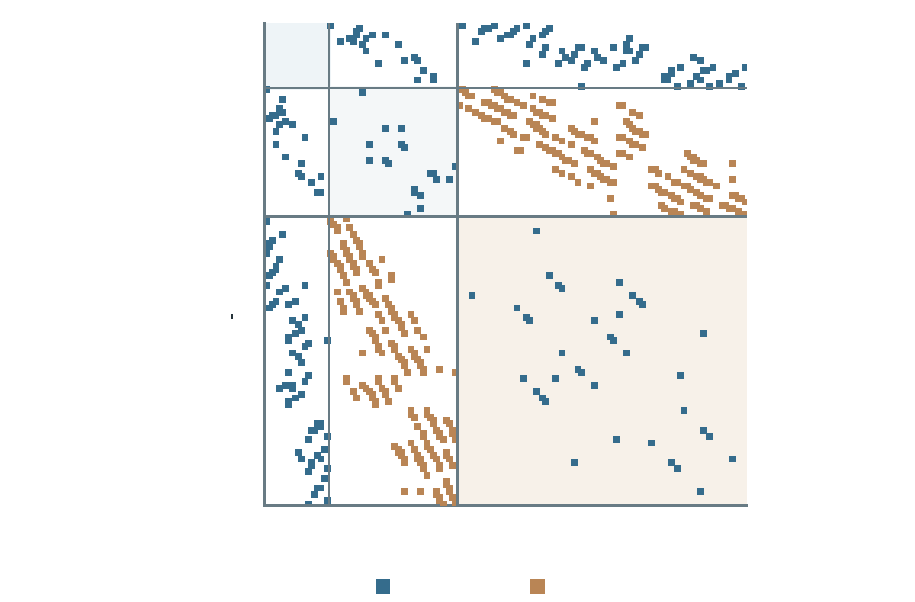
\includegraphics[width=0.86\textwidth]{figures/fig2_q1_conflict_matrix.pdf}
  \caption{问题一计划层冲突矩阵}
  \label{fig:q1-matrix}
\end{figure}

\begin{table}[H]
\centering
\caption{问题一按类别组合统计的冲突结果}
\label{tab:q1-category}
\begin{tabular}{lrrrr}
\toprule
类别组合 & 可配对数 & 冲突对数 & 类别内冲突率 & 占全部冲突对 \\
\midrule
A--A & 190 & 0 & 0.00\% & 0.00\% \\
A--B & 800 & 21 & 2.63\% & 7.07\% \\
A--C & 1\,800 & 66 & 3.67\% & 22.22\% \\
B--B & 780 & 10 & 1.28\% & 3.37\% \\
B--C & 3\,600 & 181 & 5.03\% & 60.94\% \\
C--C & 4\,005 & 19 & 0.47\% & 6.40\% \\
\midrule
合计 & 11\,175 & 297 & -- & 100.00\% \\
\bottomrule
\end{tabular}
\end{table}

表 \ref{tab:q1-category} 显示，B--C 类既贡献了最多的冲突装备对，按全部可能配对归一化后冲突率也最高。这个结果用于说明冲突结构和后续优化的输入重点，不直接规定问题二中应该移动或撤销哪些计划。

\subsubsection{问题一的检验}
独立离散资源格算法得到的 297 对冲突装备与连续半开区间算法完全一致；重新枚举事件矩形交集得到 431 次事件级重叠，与主程序一致。A001 第二次使用事件和 C083 最后一次使用事件分别通过示例语义和边界复核。输出工作簿保留附件模板的单工作表和三列字段，297 行结果与 \texttt{results.json}、\texttt{conflict\_pairs.csv} 逐行一致。

\subsubsection{问题一小结}
问题一得到的 297 条冲突边构成问题二的硬约束输入；其后的冲突消解必须重新展开每个调整动作的全部重复事件，不能只对首次事件进行局部修复。


\subsection{问题二模型的建立与求解}
\subsubsection{数据接口、候选动作与资源约束}
问题一的每条冲突边都必须在调整后的完整重复事件上重新检查。按假设（2），对每份计划 \(i\) 构造候选动作集合 \(\mathcal A_i\)，其中包含保留、频率平移、时间平移和撤销。频率平移量满足 \(\lvert\Delta f\rvert\le 10\)，时间平移量满足 \(\lvert\Delta t\rvert\le 5\)，并且一份计划不能同时改变频率和时间。所有候选动作均保持原计划的单次时长、间隔时长和使用次数不变；按假设（3）在进入模型前删除越过资源域的候选。

令 \(x_{ia}\in\{0,1\}\) 表示计划 \(i\) 是否选择动作 \(a\)，令 \(\mathcal K_{ia}\) 表示该候选动作展开后占用的离散时频资源格集合。每份计划恰选择一个候选动作：
\begin{equation}
\sum_{a\in\mathcal A_i}x_{ia}=1,\qquad i\in\mathcal I.
\label{eq:q2-one-action}
\end{equation}
对任一资源格 \(c\)，最多允许一个候选动作占用：
\begin{equation}
\sum_{(i,a):\,c\in\mathcal K_{ia}}x_{ia}\le 1.
\label{eq:q2-cell-clique}
\end{equation}
该资源格约束等价于对候选动作逐对加入冲突约束，但能够把 270\,626 条候选成对冲突边压缩为 52\,939 条资源格团约束。基准场景共形成 4\,582 个合法候选动作。

\subsubsection{条件字典序目标}
题面只给出“尽可能少撤销、少调整并优先保护高等级装备”的定性要求，直接设置任意数值权重会使结果依赖人为尺度。因此采用条件字典序
\begin{equation}
(R,\ R_A,\ R_B,\ M,\ M_A,\ M_B,\ S_{10}),
\label{eq:q2-lexicographic}
\end{equation}
逐层求解并在每层获得上下界一致或阈值不可行证据后固定该层。这里 \(R\) 为总撤销数，\(M\) 为被调整计划数，下标 \(A,B\) 表示相应类别。末级平移量定义为
\begin{equation}
S_{10}=\sum_i\left(\lvert\Delta f_i\rvert+2\lvert\Delta t_i\rvert\right)
=10\sum_i\left(\frac{\lvert\Delta f_i\rvert}{10}+
\frac{\lvert\Delta t_i\rvert}{5}\right).
\label{eq:q2-shift-score}
\end{equation}
式 \eqref{eq:q2-shift-score} 用于固定前六层后的末级并列破除；其相邻阈值不可行性也需要单独证明。

\subsubsection{模型求解与已闭合前缀}
主模型使用 CP-SAT 求解资源格约束\cite{ortools}，关键次级目标再用独立 CNF 阈值模型和 CaDiCaL\cite{cadical} 检查“更优一档是否不可行”。得到的前缀证据如下。

\begin{table}[H]
\centering
\caption{问题二条件字典序前缀的上下界证据}
\label{tab:q2-proof}
\begin{tabular}{lrrl}
\toprule
目标层 & 下界 & 上界 & 结论 \\
\midrule
总撤销 \(R\) & 6 & 6 & 已证明最优 \\
A 类撤销 \(R_A\mid R=6\) & 0 & 0 & 已证明条件最优 \\
B 类撤销 \(R_B\mid R=6,R_A=0\) & 4 & 4 & 已证明条件最优 \\
总调整 \(M\mid\text{前缀固定}\) & 126 & 126 & 已证明条件最优 \\
A 类调整 \(M_A\mid\text{前缀固定}\) & 16 & 16 & 已证明条件最优 \\
B 类调整 \(M_B\mid\text{前缀固定}\) & 34 & 34 & 已证明条件最优 \\
末级平移 \(S_{10}\mid\text{前六层固定}\) & 775 & 775 & 已证明条件最优 \\
\bottomrule
\end{tabular}
\end{table}

因此，当前已证明的完整条件字典序结果为
\[
(R,R_A,R_B,M,M_A,M_B,S_{10})=(6,0,4,126,16,34,775).
\]
其中 \(R\) 的上下界来自 CP-SAT 的最优证书；B 类撤销数、三层调整数和末级平移量的下界由独立 CNF 阈值不可行证明给出。末级证书在完整 4\,582 个候选动作全集上检验 \(S_{10}\le774\) 不可行。

表 \ref{tab:q2-proof} 已经完整给出每一层的上下界和证明状态，因此不再另设证明阶梯图，避免用图形重复同一组离散证据。

\subsubsection{六撤销方案与结果}
在上述前缀下得到的正式方案按类别统计如下。

\begin{table}[H]
\centering
\caption{问题二正式方案的类别构成}
\label{tab:q2-solution}
\begin{tabular}{lrrr}
\toprule
类别 & 保留 & 调整 & 撤销 \\
\midrule
A & 4 & 16 & 0 \\
B & 2 & 34 & 4 \\
C & 12 & 76 & 2 \\
\midrule
合计 & 18 & 126 & 6 \\
\bottomrule
\end{tabular}
\end{table}

撤销计划为 B009、B018、B024、B028、C027 和 C054。方案保留 144 个活动计划，占用 15\,816 个不同资源格；频移绝对值总和为 595，时移绝对值总和为 90，因而当前方案的 \(S_{10}=775\)。

图 \ref{fig:q2-composition} 展示同一动作表的类别构成。A 类没有撤销，B 类承担 4 次撤销，C 类保留 12 条、调整 76 条并撤销 2 条；这张图只用于呈现动作组成，不替代前缀证明。

\begin{figure}[htbp]
  \centering
  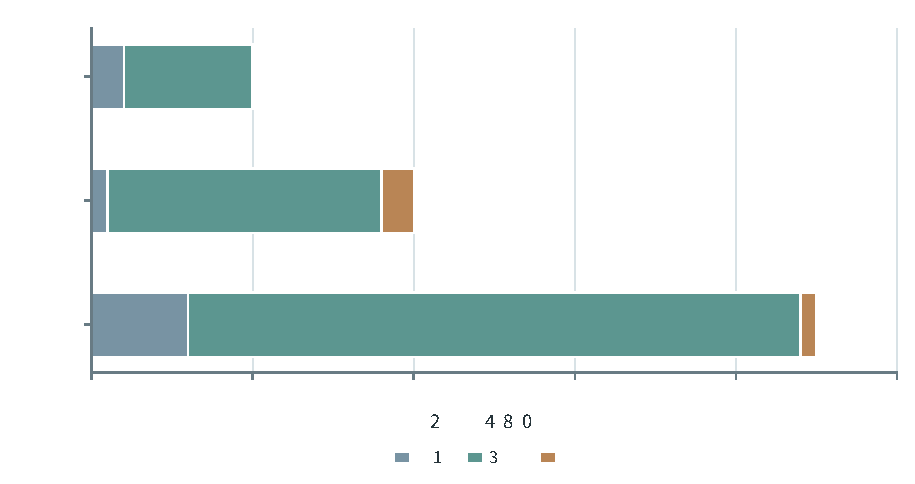
\includegraphics[width=0.88\textwidth]{figures/fig4_q2_composition.pdf}
  \caption{问题二正式方案的类别构成}
  \label{fig:q2-composition}
\end{figure}

\subsubsection{独立可行性检验}
验证程序从动作表重新读取原始附件，并分别用连续半开区间和离散资源格复核全部重复事件。两种方法均得到零冲突、零越界和零重复占用，最大单元占用数为 1。结果工作簿只填写发生变化的参数列，132 条动作行通过工作簿格式检查。该六撤销方案作为问题三的冻结输入，不由问题三的新增容量反向修改。

\subsubsection{最优性边界}
末级平移量也已闭合：在固定 \((R,R_A,R_B,M,M_A,M_B)=(6,0,4,126,16,34)\) 后，完整候选全集上的独立 CNF 模型返回 \(S_{10}\le774\) 为 \texttt{UNSAT}；正式方案给出 \(S_{10}=775\)，故末级上下界一致。该结论只针对本文明确的有限动作集合、半开区间和 \(H=643\) 资源域。

\subsubsection{问题二小结}
问题二把 Q1 的冲突边转化为候选动作之间的资源格互斥关系，得到总撤销数为 6 的已验证方案，并对高层目标、类别保护目标和末级平移量均给出上下界证据。


\subsection{问题三模型的建立与求解}
\subsubsection{固定背景与候选集合}
按假设（3），问题三读取经验证的问题二工作簿，固定其中 144 个活动计划和 15\,816 个已占用资源格，不在本问重新平移或撤销原计划。新增 C 类计划继承附件中的共同结构：频段宽度为 3，单次时长为 2，间隔时长为 8，使用次数为 12，因此相邻起点步长为 10。每个完整 C 类候选计划占用 \(3\times2\times12=72\) 个离散时频资源格。

在资源域 \([0,643)\times[0,100)\) 内，频段起点和首次时间起点分别满足
\[
f_0=0,1,\ldots,97,\qquad t_0=0,1,\ldots,531.
\]
因此完整候选起点总数为 \(98\times532=52\,136\)。逐个展开候选的 12 次使用事件并与固定问题二背景比较后，保留 2\,334 个无冲突候选。候选筛选没有抽样，也没有用剩余面积除以 72 代替完整模板检查。

图 \ref{fig:q3-candidate-layout} 用起点坐标展示这一筛选结果：浅色点是与冻结 Q2 背景不冲突的 2\,334 个候选，深色点是最终选中的 141 个新增计划。图中位置只表示候选起点，不把起点密度误读为优化目标。

\begin{figure}[htbp]
  \centering
  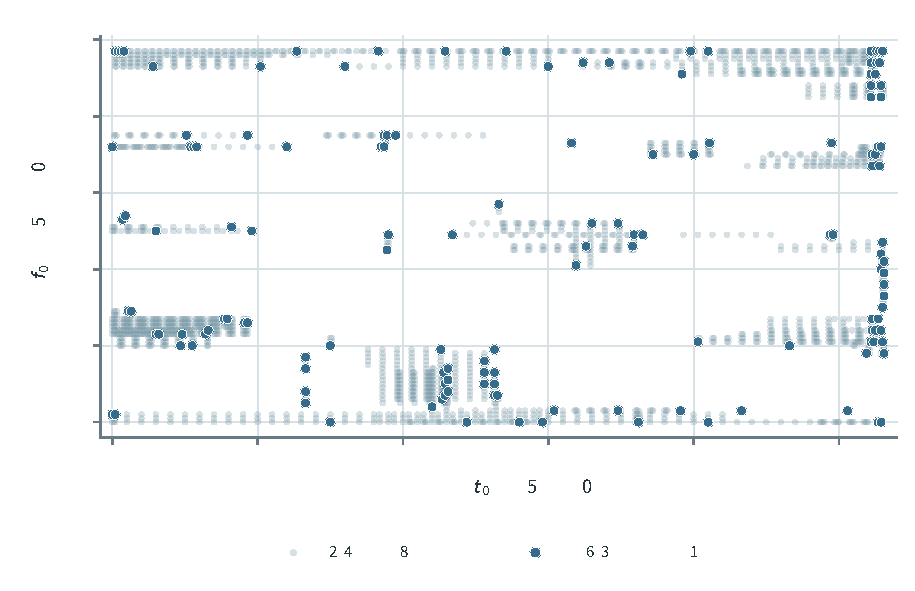
\includegraphics[width=0.92\textwidth]{figures/fig5_q3_candidate_layout.pdf}
  \caption{固定问题二条件下的 C 类候选起点与选中方案}
  \label{fig:q3-candidate-layout}
\end{figure}

\subsubsection{集合装填模型}
对每个合法候选 \(p\) 定义二元变量 \(y_p\)，令 \(\mathcal K_p\) 为其完整资源格集合，最大化新增计划数量：
\begin{equation}
\max\sum_{p}y_p,
\qquad
\sum_{p:\,c\in\mathcal K_p}y_p\le 1-O_c,
\quad c\in\mathcal C,
\label{eq:q3-set-packing}
\end{equation}
其中 \(O_c\) 表示固定问题二方案对资源格 \(c\) 的占用。主模型包含 2\,334 个候选变量、15\,521 条被候选使用的资源格约束和 168\,048 个非零系数。

\subsubsection{最大新增数量}
集合装填模型返回 141 个新增计划，HiGHS 求解器\cite{highs} 状态为 \texttt{OPTIMAL}，下界和上界均为 141，MIP gap 为 0。为避免结论依赖单一约束编码，又将 2\,334 个候选改写为候选两两冲突模型；若两个候选共享任一资源格，则加入
\[
y_p+y_q\le 1.
\]
该独立模型含 66\,472 条成对冲突约束，同样得到 141。进一步加入 \(\sum_p y_p\ge142\) 后模型不可行，因此“141 台可行”和“142 台不可行”共同闭合了固定背景下的最大新增数量。

\begin{table}[H]
\centering
\caption{问题三候选筛选与最大性验证}
\label{tab:q3-result}
\begin{tabular}{lr}
\toprule
项目 & 数值 \\
\midrule
完整 C 类候选起点 & 52\,136 \\
与固定 Q2 背景不冲突的候选 & 2\,334 \\
集合装填模型下界/上界 & 141/141 \\
独立成对冲突模型下界/上界 & 141/141 \\
新增计划数 & 141 台 \\
\bottomrule
\end{tabular}
\end{table}

\subsubsection{合并结果与边界}
141 台新增计划占用 10\,152 个资源格，与固定问题二方案合并后形成 285 个活动计划，占用 25\,968 个不同资源格。连续半开区间检查和离散资源格检查均未发现 Q2--Q3 间冲突或新增计划之间的冲突，\texttt{result3.xlsx} 的 141 行与结果 JSON 逐行一致。

“最多新增 141 台”依赖三个条件：当前批准的具体问题二方案、资源域 \([0,643)\times[0,100)\) 以及附件 C 类共同模板。改变任一条件都需要重新生成候选集合并求解，不能将 141 台推广到任意问题二方案。

\subsubsection{问题三小结}
在固定问题二方案下，完整候选枚举与两种独立冲突编码均支持最多新增 141 台 C 类装备；该结果是条件最优结论，且其适用边界已经明确。


\subsection{问题四模型的建立与求解}
\subsubsection{问题四的数据接口与有限动作集合}

问题四从问题一的 150 条原始计划重新开始，不读取问题二的工作簿作为约束，也不把问题三新增的 C 类计划混入本问。基准资源域仍为 \([0,643)\times[0,100)\)，事件采用半开区间，所有时间端点和调整量按整数资源单位处理。

每份计划只能选择一种动作。A、B、C 三类均可保持、频率平移、首次时间平移或撤销；C 类额外允许改变重复使用之间的空闲间隔。频率平移量和首次时间平移量分别满足
\[
\delta f\in\{-10,\ldots,-1,1,\ldots,10\},\qquad
\delta t\in\{-5,\ldots,-1,1,\ldots,5\}.
\]
对 C 类计划，令原空闲间隔为 \(g_i=8\)，间隔调整量为
\[
\delta g\in\{-8,\ldots,-1,1,\ldots,10\},
\qquad g_i'=8+\delta g\in\{0,1,\ldots,18\}.
\]
选择间隔动作时，频段区间和首次时间区间保持原值；选择频率或时间平移动作时，\(\delta g=0\)。使用次数、频段宽度和单次占用时长均不改变。

\subsubsection{间隔调整下的重复事件递推}

若计划 \(i\) 的首次时间区间为 \([s_i,e_i)\)，单次占用时长为 \(l_i=e_i-s_i\)，调整后的空闲间隔为 \(g_i'\)，则第 \(k\) 次事件为
\begin{equation}
T_{ik}(g_i')=
\left[s_i+k(l_i+g_i'),\ e_i+k(l_i+g_i')\right),
\qquad k=0,1,\ldots,n_i-1.
\label{eq:q4-event-expansion}
\end{equation}
间隔变化会联动第二次及以后的全部事件，因此每个候选动作先完整展开，再进行边界和资源格检查；不以单个事件平移或平均占用替代完整递推。

\subsubsection{问题四资源格模型与目标}

令 \(\mathcal A_i^{(4)}\) 为计划 \(i\) 的 Q4 合法动作集合，令 \(x_{ia}\in\{0,1\}\) 表示是否选择动作 \(a\)，令 \(\mathcal K_{ia}^{(4)}\) 表示该动作的完整重复事件占用的离散时频资源格集合。每份计划恰选择一种动作：
\begin{equation}
\sum_{a\in\mathcal A_i^{(4)}}x_{ia}=1,
\qquad i\in\mathcal I.
\label{eq:q4-one-action}
\end{equation}
对每个资源格 \(c\)，加入
\begin{equation}
\sum_{(i,a):\,c\in\mathcal K_{ia}^{(4)}}x_{ia}\le 1,
\qquad c\in\mathcal C.
\label{eq:q4-cell-clique}
\end{equation}
该约束保证所有未撤销计划的完整事件在两个维度上均无冲突。基准场景共生成 6\,103 个合法候选动作，其中 5\,953 个为活动候选；按同一计划的外部冲突集合做支配消元后保留 5\,533 个活动候选。420 个被消去动作均有同计划、外部冲突集合为其子集的保留动作，支配替换核验通过。

为保持与问题二相同的优先级口径，Q4 仍按
\[
R\rightarrow R_A\rightarrow R_B\rightarrow M\rightarrow M_A\rightarrow M_B\rightarrow S_{10}^{(4)}
\]
比较，其中前六层分别表示撤销和调整计划数，末级候选指标为
\begin{equation}
S_{10}^{(4)}=\sum_i\left(|\delta f_i|+2|\delta t_i|+|\delta g_i|\right).
\label{eq:q4-shift-score}
\end{equation}
本阶段只闭合决定方案规模的最小撤销层；\(R=3\) 内的部分次级目标仍以条件候选记录，不写成完整字典序最优。

\subsubsection{最小撤销数的上下界证明}

首先由 \texttt{proof\_R\_le\_3.json} 构造 3 台撤销的无冲突方案，并通过连续半开区间、离散资源格和独立重建检查。因此得到可行上界 \(R\le3\)。

为证明 \(R\le2\) 不可行，若存在少于 2 台撤销的可行方案，可以再撤销任意计划补足到恰好 2 台，且撤销不会制造新的资源冲突，故只需考察恰好 2 台撤销。两台撤销在 A、B、C 三类之间只有
\[
(0,0,2),(0,1,1),(0,2,0),(1,0,1),(1,1,0),(2,0,0)
\]
六种类别分拆。对六个分支分别保留全部计划身份和合法活动动作，建立 \(R=2\) 的 SAT 判定模型；六个分支均返回 \texttt{UNSAT}。分支覆盖和支配消元均由独立核验文件检查通过，因此 \(R\le2\) 在本文有限动作集合内不可行。该阈值核验采用 CaDiCaL\cite{cadical}，但其输入候选全集和资源口径与主模型相同。结合 3 台可行见证，得到
\begin{equation}
R_{Q4}^{\ast}=3.
\label{eq:q4-min-revoke}
\end{equation}
这里的结论只针对整数时频资源格、\(H=643\) 和上述有限动作集合，不外推到连续调整或未列出的动作。

\begin{table}[H]
\centering
\caption{问题四最小撤销层的证据状态}
\label{tab:q4-proof}
\begin{tabular}{lccc}
\toprule
检验层 & 方案/阈值 & 证据状态 & 允许的结论 \\
\midrule
可行上界 & \(R\le3\) & 可行且独立验证通过 & 3 台撤销可行 \\
全局下界 & \(R\le2\) & 六个类别分支均 \texttt{UNSAT} & 2 台及以下不可行 \\
最小撤销层 & \(R=3\) & 上下界闭合 & 当前有限模型下最小撤销数为 3 \\
\bottomrule
\end{tabular}
\end{table}

\subsubsection{当前条件候选与工作簿核验}

在固定 \(R=3\)、\(R_A=0\)、\(R_B=1\) 的条件下，当前候选链给出 142 个调整计划，但 \(R_B=1\)、\(M=142\) 和 \(S_{10}^{(4)}=943\) 尚未全部完成相邻阈值不可行证明。用于生成 \texttt{result4.xlsx} 的同一候选方案统计如下。

\begin{table}[H]
\centering
\caption{问题四当前条件可行方案的类别构成}
\label{tab:q4-candidate}
\begin{tabular}{lrrr}
\toprule
类别 & 保留 & 调整 & 撤销 \\
\midrule
A & 0 & 20 & 0 \\
B & 0 & 39 & 1 \\
C & 5 & 83 & 2 \\
\midrule
合计 & 5 & 142 & 3 \\
\bottomrule
\end{tabular}
\end{table}

该工作簿撤销 B029、C035、C075，共有 147 个活动计划。独立回读重新计算得到 16\,356 个不同占用资源格，连续冲突数、离散冲突数和越界数均为 0，最大资源格占用数为 1，工作簿报告值与重算值一致。表 \ref{tab:q4-candidate} 只描述当前条件可行候选，不把 142 或 943 写成次级全局最优。

\subsubsection{边界敏感性与问题四小结}

在 \(H=638,643,648\) 三个时间域右端点下，均找到通过独立验证的 \(R\le3\) 候选，候选动作数分别为 6\,040、6\,103 和 6\,116，资源格约束数分别为 53\,186、53\,679 和 53\,767。该检验支持“3 台撤销可行上界对边界扰动稳定”，不宣称两个敏感性域的最小撤销数也已经闭合。

问题四在 Q2 的动作框架上只增加 C 类间隔调整，间隔变化通过完整重复事件递推进入资源格约束。六分支不可行证明与三撤销可行见证闭合了当前有限模型下的最小撤销层；其后的类别撤销、调整数量和末级变化量仍需与证据状态一起表述。


\section{模型检验}
\subsection{独立编码一致性}
问题一使用连续半开区间算法和离散时频单元倒排算法交叉检查；问题二对调整后的全部重复事件进行连续区间与离散资源格复核；问题三同时使用资源格集合装填和候选两两冲突两种编码；问题四对候选工作簿重新展开，并分别用连续区间、离散资源格和独立重建程序复核。四个问题的主要结果分别为 297 对、零冲突六撤销方案、141 台最大新增和三撤销可行见证，独立编码没有产生不一致。

\subsection{问题二的时间域敏感性}
\label{sec:q2-sensitivity}
统一时间域的右端点 643 来自完整数据展开。为检查该数据驱动边界是否决定撤销数量，分别考察 \(H=638,643,648\) 三个情景。每个情景都重新筛选越界候选，并对“总撤销数不超过 5”进行不可行检验，同时验证六撤销见证的边界和冲突状态。

\begin{table}[H]
\centering
\caption{不同时间域右端点下的最小撤销数}
\label{tab:q2-horizon}
\begin{tabular}{lrrl}
\toprule
时间域右端点 \(H\) & 候选动作数 & 最小撤销数 & 验证状态 \\
\midrule
638 & 4\,528 & 6 & 下界与见证均通过 \\
643 & 4\,582 & 6 & 基准方案通过 \\
648 & 4\,589 & 6 & 下界与宽域见证均通过 \\
\bottomrule
\end{tabular}
\end{table}

三个情景均得到最小撤销数 6，说明主目标对该范围内的时间边界扰动不敏感。但这项检验只支持“最小撤销数保持为 6”，不表示三个情景下的完整字典序末级平移量都已经证明最优。

表 \ref{tab:q2-horizon} 已经同时列出三个边界情景的候选动作数、最小撤销数和验证状态，足以支持该项敏感性结论，因此不再用图形重复表格。

\subsection{问题三的最大性复核}
问题三的集合装填模型和候选两两冲突模型分别得到 141 的上下界；增加 142 台阈值约束后返回不可行。该复核针对问题三的唯一主目标，且独立于问题二末级平移量的未闭合状态。

\subsection{问题四的候选覆盖与最小撤销层}
问题四先对有限动作全集做边界筛选，再检查支配替换的覆盖性。基准域内共有 6\,103 个合法候选动作，其中 5\,953 个为活动候选；支配消元保留 5\,533 个，删除的 420 个动作均能由同计划保留动作替换，候选覆盖核验通过。三撤销见证由连续区间、离散资源格和独立重建共同复核；对 $R=2$ 的六种类别分拆逐支建立阈值判定，六支均返回不可行。因此，$R_{Q4}^{\ast}=3$ 的最小撤销层在当前有限模型内形成上下界闭合。

\subsection{问题四条件候选与边界检查}
用于论文展示的条件候选含 147 个活动计划和 16\,356 个不同占用资源格；连续冲突、离散冲突和越界数均为 0，最大资源格占用数为 1，工作簿报告值与独立重算值一致。候选类别统计为 A 类 $0/20/0$、B 类 $0/39/1$、C 类 $5/83/2$（保留/调整/撤销），但 $R_B=1$、$M=142$ 和 $S_{10}^{(4)}=943$ 的相邻次级不可行证据尚未全部闭合，因此只作为条件候选呈现。进一步在 $H=638,643,648$ 下均找到通过验证的三撤销候选，支持可行上界对边界扰动稳定，不把两个敏感性域的最小值误写成已证明结论。

\subsection{跨问题接口检查}
问题三只读取问题二的冻结工作簿，不通过新增容量反向修改问题二；问题四则从问题一的原始 150 条计划独立起算，不读取 Q2/Q3 的批准或新增结果。合并验证同时检查资源边界、Q2--Q3 冲突、Q3 内部冲突、Q4 全量重复事件、重复资源格和输出工作簿行数，全部通过。因而四问结果形成“共同预处理—按问求解—按问复核”的单向证据链。


\section{模型优缺点评价}
\subsection{模型的优点}
\begin{enumerate}[label=(\arabic*)]
  \item 统一将周期性计划展开为完整重复事件，避免只检查首次时间区间造成漏检。
  \item 用离散时频资源格表达冲突，使 Q2 和 Q3 的可行性能够由独立程序复核。
  \item 对问题二的主要优先级采用条件字典序，并对关键阈值给出上下界或不可行证据，避免把限时可行解直接称为全局最优。
  \item 问题四只增加 C 类间隔调整这一项自由度，并将其通过完整事件递推接入同一资源格模型；三撤销见证、六分支不可行证据和支配覆盖核验使最小撤销层具有可审计的上下界结构。
\end{enumerate}

\subsection{模型的缺点}
\begin{enumerate}[label=(\arabic*)]
  \item 统一时间域右端点 643 是由当前附件展开得到的数据驱动边界，题面没有直接给出该全局终点；虽然进行了 \(H=638,643,648\) 敏感性检验，外推到更宽时间域仍需重新求解。
  \item 问题二末级归一化平移量 \(S_{10}\) 尚未完成全局最小性证明，当前方案的 775 只能作为可行上界。
  \item 问题三的 141 台结果依赖当前 Q2 方案和附件 C 类共同模板，不能直接推广到其他 Q2 背景或其他新增计划结构。
  \item 问题四的 \(R_{Q4}^{\ast}=3\) 只对给定整数动作集合和 \(H=643\) 闭合了最小撤销层；当前 \(R_B=1\)、\(M=142\) 和 \(S_{10}^{(4)}=943\) 尚未完成全部相邻层的不可行证明，不能作为完整字典序最优结论。
\end{enumerate}

\subsection{模型的改进}
后续可在保持资源格精确约束的基础上继续完成 Q2 的 \(S_{10}\) 与 Q4 次级字典序层的阈值证明，并在 \(H=638,648\) 情景下补做最小撤销数的下界核验。若进一步放宽间隔、频率或时间动作，必须重新生成全部候选事件、资源格和跨问接口，而不能在已有工作簿上做局部修补。


\section*{AI 工具使用声明}
本参赛队在竞赛过程中使用了 AI 工具，主要用于论文语言与版式整理、代码调试辅助、结果证据核对和图表/排版检查，详细使用情况见支撑材料中的“AI 工具使用详情.pdf”。

\clearpage
\section*{参考文献}
\renewcommand{\refname}{}
\begin{thebibliography}{99}
\bibitem{ortools}
Google OR-Tools. CP-SAT Solver[EB/OL]. Google for Developers, 2026-09-12.\
\url{https://developers.google.com/optimization/cp/cp_solver}.

\bibitem{highs}
Huangfu Q, Hall J A J. Parallelizing the dual revised simplex method[J]. Mathematical Programming Computation, 2018, 10(1): 119--142. DOI:10.1007/s12532-017-0130-5.

\bibitem{cadical}
Biere A, Faller T, Fazekas K, Fleury M, Froleyks N, Pollitt F. CaDiCaL 2.0[C]//Gurfinkel A, Ganesh V, eds. Computer Aided Verification. Lecture Notes in Computer Science, vol. 14681. Cham: Springer, 2024: 133--152. DOI:10.1007/978-3-031-65627-9\_7.
\end{thebibliography}

\clearpage
\section*{附录}
\begin{itemize}
  \item 支撑材料压缩包：\texttt{支撑材料\_Q4完整稿\_20260912.zip}，其中包含可运行源程序、结果文件、验证证据、版本与复核说明。
  \item AI 工具使用详情：支撑包根目录下的\texttt{AI 工具使用详情.pdf}，记录工具名称、使用目的、提示方式、人工修改和核验情况。
  \item 问题一：冲突清单、结果工作簿、独立复核输出和绘图数据位于支撑包的 Q1 输出目录 \texttt{outputs/q1/}。
  \item 问题二：正式动作表、前缀证明矩阵、SAT 阈值证据和验证输出位于\texttt{outputs/q2/}；\(S_{10}=775\) 只标记为已闭合前缀下的可行上界。
  \item 问题三：批准 Q2 接口、候选结果、141 台最大性审计和验证输出位于\texttt{outputs/q3/}；结论范围为固定 Q2 背景。
  \item 问题四：三撤销可行见证、六分支 \texttt{UNSAT} 证据、支配替换核验、当前条件候选和\texttt{result4.xlsx} 位于\texttt{outputs/q4/}；\(R=3\) 已证明为最小撤销层，次级层仍按状态标注。
  \item 题目提供的原始附件不在支撑包中重复分发；程序 README 记录了文件名、期望路径和 SHA-256 核对方式。
\end{itemize}

\end{document}
